% ========================================
%	Header einbinden
% ========================================

\documentclass[bibtotoc,titlepage]{scrartcl}

% Deutsche Spracheinstellungen
\usepackage[ngerman,german]{babel, varioref}
\usepackage[T1]{fontenc}
\usepackage[utf8]{inputenc}

%\usepackage{marvosym}

\usepackage{amsfonts}
\usepackage{amssymb}
\usepackage{amsmath}
\usepackage{amscd}
\usepackage{amstext}

\usepackage{longtable}

%\usepackage{bibgerm}

\usepackage{footnpag}

\usepackage{ifthen}                 %%% package for conditionals in TeX
\usepackage[amssymb]{SIunits}
%Für textumflossene Bilder und Tablellen
%\usepackage{floatflt} - veraltet

%Für Testzwecke aktivieren, zeigt labels und refs im Text an.
%\usepackage{showkeys}

% Abstand zwischen zwei Absätzen nach DIN (1,5 Zeilen)
% \setlength{\parskip}{1.5ex plus0.5ex minus0.5ex}

% Einrückung am Anfang eines neuen Absatzes nach DIN (keine)
%\setlength{\parindent}{0pt}

% Ränder definieren
% \setlength{\oddsidemargin}{0.3cm}
% \setlength{\textwidth}{15.6cm}

% bessere Bildunterschriften
%\usepackage[center]{caption2}


% Problemlösungen beim Umgang mit Gleitumgebungen
\usepackage{float}

% Nummeriert bis zur Strukturstufe 3 (also <section>, <subsection> und <subsubsection>)
%\setcounter{secnumdepth}{3}

% Führt das Inhaltsverzeichnis bis zur Strukturstufe 3
%\setcounter{tocdepth}{3}
\usepackage[version=3]{mhchem}
	\mhchemoptions{minus-sidebearing-left=0.06em, minus-sidebearing-right=0.11em}
\usepackage{exscale}

\newenvironment{dsm} {\begin{displaymath}} {\end{displaymath}}
\newenvironment{vars} {\begin{center}\scriptsize} {\normalsize \end{center}}


\newcommand {\en} {\varepsilon_0}               % Epsilon-Null aus der Elektrodynamik
\newcommand {\lap} {\; \mathbf{\Delta}}         % Laplace-Operator
\newcommand {\R} { \mathbb{R} }                 % Menge der reellen Zahlen
\newcommand {\e} { \ \mathbf{e} }               % Eulersche Zahl
\renewcommand {\i} { \mathbf{i} }               % komplexe Zahl i
\newcommand {\N} { \mathbb{N} }                 % Menge der nat. Zahlen
\newcommand {\C} { \mathbb{C} }                 % Menge der kompl. Zahlen
\newcommand {\Z} { \mathbb{Z} }                 % Menge der kompl. Zahlen
\newcommand {\limi}[1]{\lim_{#1 \rightarrow \infty}} % Limes unendlich
\newcommand {\sumi}[1]{\sum_{#1=0}^\infty}
\newcommand {\rot} {\; \mathrm{rot} \,}         % Rotation
\newcommand {\grad} {\; \mathrm{grad} \,}       % Gradient
\newcommand {\dive} {\; \mathrm{div} \,}        % Divergenz
\newcommand {\dx} {\; \mathrm{d} }              % Differential d
\newcommand {\cotanh} {\; \mathrm{cotanh} \,}   %Cotangenshyperbolicus
\newcommand {\asinh} {\; \mathrm{areasinh} \,}  %Area-Sinus-Hyp.
\newcommand {\acosh} {\; \mathrm{areacosh} \,}  %Area-Cosinus-H.
\newcommand {\atanh} {\; \mathrm{areatanh} \,}  %Area Tangens-H.
\newcommand {\acoth} {\; \mathrm{areacoth} \,}  % Area-cotangens
\newcommand {\Sp} {\; \mathrm{Sp} \,}
\newcommand {\mbe} {\stackrel{\text{!}}{=}}     %Must Be Equal
\newcommand{\qed} { \hfill $\square$\\}
\renewcommand{\i} {\imath}
\def\captionsngerman{\def\figurename{\textbf{Abb.}}}

%%%%%%%%%%%%%%%%%%%%%%%%%%%%%%%%%%%%%%%%%%%%%%%%%%%%%%%%%%%%%%%%%%%%%%%%%%%%
% SWITCH FOR PDFLATEX or LATEX
%%%%%%%%%%%%%%%%%%%%%%%%%%%%%%%%%%%%%%%%%%%%%%%%%%%%%%%%%%%%%%%%%%%%%%%%%%%%
%%%
\ifx\pdfoutput\undefined %%%%%%%%%%%%%%%%%%%%%%%%%%%%%%%%%%%%%%%%% LATEX %%%
%%%
\usepackage[dvips]{graphicx}       %%% graphics for dvips
\DeclareGraphicsExtensions{.eps,.ps}   %%% standard extension for included graphics
\usepackage[ps2pdf]{thumbpdf}      %%% thumbnails for ps2pdf
\usepackage[ps2pdf,                %%% hyper-references for ps2pdf
bookmarks=true,%                   %%% generate bookmarks ...
bookmarksnumbered=true,%           %%% ... with numbers
hypertexnames=false,%              %%% needed for correct links to figures !!!
breaklinks=true,%                  %%% breaks lines, but links are very small
linkbordercolor={0 0 1},%          %%% blue frames around links
pdfborder={0 0 112.0}]{hyperref}%  %%% border-width of frames
%                                      will be multiplied with 0.009 by ps2pdf
%
\hypersetup{ pdfauthor   = {Hannes Franke; Julius Tilly},
pdftitle    = {V301 Innenwiderstand und Leistungsanpassung}, pdfsubject  = {Protokoll FP}, pdfkeywords = {V301, Innenwiderstand, Leistungsanpassung},
pdfcreator  = {LaTeX with hyperref package}, pdfproducer = {dvips
+ ps2pdf} }
%%%
\else %%%%%%%%%%%%%%%%%%%%%%%%%%%%%%%%%%%%%%%%%%%%%%%%%%%%%%%%%% PDFLATEX %%%
%%%
\usepackage[pdftex]{graphicx}      %%% graphics for pdfLaTeX
\DeclareGraphicsExtensions{.pdf}   %%% standard extension for included graphics
\usepackage[pdftex]{thumbpdf}      %%% thumbnails for pdflatex
\usepackage[pdftex,                %%% hyper-references for pdflatex
bookmarks=true,%                   %%% generate bookmarks ...
bookmarksnumbered=true,%           %%% ... with numbers
hypertexnames=false,%              %%% needed for correct links to figures !!!
breaklinks=true,%                  %%% break links if exceeding a single line
linkbordercolor={0 0 1},
linktocpage]{hyperref} %%% blue frames around links
%                                  %%% pdfborder={0 0 1} is the default
\hypersetup{
pdftitle    = {V301 Innenwiderstand und Leistungsanpassung}, 
pdfsubject  = {Protokoll AP}, 
pdfkeywords = {V301, Innenwiderstand, Leistungsanpassung},
pdfsubject  = {Protokoll AP},
pdfkeywords = {V301, Innenwiderstand, Leistungsanpassung}}
%                                  %%% pdfcreator, pdfproducer,
%                                      and CreationDate are automatically set
%                                      by pdflatex !!!
\pdfadjustspacing=1                %%% force LaTeX-like character spacing
\usepackage{epstopdf}
%
\fi %%%%%%%%%%%%%%%%%%%%%%%%%%%%%%%%%%%%%%%%%%%%%%%%%%% END OF CONDITION %%%
%%%%%%%%%%%%%%%%%%%%%%%%%%%%%%%%%%%%%%%%%%%%%%%%%%%%%%%%%%%%%%%%%%%%%%%%%%%%
% seitliche Tabellen und Abbildungen
%\usepackage{rotating}
\usepackage{ae}
\usepackage{
  array,
  booktabs,
  dcolumn
}
\makeatletter 
  \renewenvironment{figure}[1][] {% 
    \ifthenelse{\equal{#1}{}}{% 
      \@float{figure} 
    }{% 
      \@float{figure}[#1]% 
    }% 
    \centering 
  }{% 
    \end@float 
  } 
  \makeatother 


  \makeatletter 
  \renewenvironment{table}[1][] {% 
    \ifthenelse{\equal{#1}{}}{% 
      \@float{table} 
    }{% 
      \@float{table}[#1]% 
    }% 
    \centering 
  }{% 
    \end@float 
  } 
  \makeatother 
%\usepackage{listings}
%\lstloadlanguages{[Visual]Basic}
%\allowdisplaybreaks[1]
%\usepackage{hycap}
%\usepackage{fancyunits}


% ========================================
%	Angaben für das Titelblatt
% ========================================

\title{Versuch 501/2 -Ablenkung eines Elektronenstrahls im elektrischen Feld und im transversalen Magnetfeld\\				% Titel des Versuchs 
\large TU Dortmund, Fakultät Physik\\ 
\normalsize Anfänger-Praktikum}

\author{Jan Adam\\			% Name Praktikumspartner A
{\small \href{jan.adam@tu-dortmund.de}{jan.adam@tu-dortmund.de}}	% Erzeugt interaktiven einen Link
\and						% um einen weiteren Author hinzuzfügen
Dimitrios Skodras\\					% Name Praktikumspartner B
{\small \href{dimitrios.skodras@tu-dortmund.de}{dimitrios.skodras@tu-dortmund.de}}		% Erzeugt interaktiven einen Link
}
\date{06.November 2012}				% Das Datum der Versuchsdurchführung

% ========================================
%	Das Dokument beginnt
% ========================================

\begin{document}

% ========================================
%	Titelblatt erzeugen
% ========================================

\maketitle					% Jetzt wird die Titelseite erzeugt
\thispagestyle{empty} 				% Weder Kopfzeile noch Fußzeile

% ========================================
%	Der Vorspann
% ========================================

%\newpage					% Wenn Verzeichnisse auf einer neuen Seite beginnen sollen
%\pagestyle{empty}				% Weder Kopf- noch Fußzeile für Verzeichnisse

\tableofcontents

%\newpage					% eine neue Seite
%\thispagestyle{empty}				% Weder Kopf- noch Fußzeile für Verzeichnisse
%\listoffigures					% Abbildungsverzeichnis

%\newpage					% eine neue Seite
%\thispagestyle{empty}				% Weder Kopf- noch Fußzeile für Verzeichnisse
%\listoftables					% Tabellenverzeichnis
\newpage					% eine neue Seite


% ========================================
%	Kapitel
% ========================================

\section{Einleitung}				% Bei Bedarf

\section{Theorie}

\section{Durchführung}

\section{Auswertung}

\subsection{Proportionalität zwischen Verschiebung und Ablenkspannung}

\renewcommand{\arraystretch}{1.5}
\begin{table}[h]
\begin{tabular}{c|ccccc}
\centering
  & $U_b$ = 225 V &  $U_b$ = 300 V &  $U_b$ = 350 V &  $U_b$ = 400 V &  $U_b$ = 450 V\\
 \hline
 D[cm] & $U_d$[V] & $U_d$[V] & $U_d$[V] & $U_d$[V] & $U_d$[V]\\
 \hline
-1,429	&-9,08	&-11,98	&-15,2	&-16,9&	-19,9\\
-0,794	&-5,31	&-6,08	&-9,3	&-9,8&	-11,5\\
-0,159	&-0,79	&-0,31	&-2,02	&-1,18&	-2,82\\
0,476	&3,30	&5,35	&4,81	&6,24&	6,57\\
1,111	&7,65	&10,91	&11,31	&13,47&	15,07\\
1,746	&11,70	&16,61	&17,93	&20,9	&23,6\\
2,381	&16,03	&21,9	&24,6	&28,8	&31,5\\
3,016	&20,5	&27,4	&31,0	&35,1	&n.D\\
3,651	&24,1	&32,4	&n.D	&n.D	&n.D\\
 \end{tabular}
\label{PropUD}
\centering
\caption{Leuchtfleckverschiebung durch Ablenkspannungen bei verschiedenen Beschleunigungsspannungen}
\end{table}
\renewcommand{\arraystretch}{1}

Aus Tabelle \eqref{PropUD} ist ersichtlich, dass die Größen D und $U_d$ linear abhängig sind. Durch lineare Regression, 
ausgeführt mit GNUPLOT ergeben sich die Steigungen $a = \frac{D}{U_d}$ für die fünf Beschleunigungsspannungen. Bei 
Gegenüberstellung der Empfindlichkeit $a$ und dem Kehrwert zur jeweiligen Beschleunigungsspannung wird ebenfalls eine
lineare Abhängigkeit deutlich.


\renewcommand{\arraystretch}{1.5}
\begin{table}[h]
 \begin{tabular}{c|c|c}
  $\frac{1}{U_b}$[$\frac1V$] & a[$\frac{cm}{V}$] & $\Delta$ a[$\frac{cm}{V}$] \\
  \hline
  $4.444 \cdot 10^{-3}$ & 0,1497 & 0,00102 \\
  $3.333 \cdot 10^{-3}$ & 0,1105 & 0,00184 \\
  $2.857 \cdot 10^{-3}$ & 0,0964 & 0,00095 \\
  $2.500 \cdot 10^{-3}$ & 0,0841 & 0,00078 \\
  $2.222 \cdot 10^{-3}$ & 0,0739 & 0,00085 \\
 \end{tabular}
\label{propUa}
\caption{Empfindlichkeit a gegenüber der inversen Beschleunigungsspannung}
\end{table}
\renewcommand{\arraystretch}{1}

Durch Ausgleichsrechnung zwischen der inversen Beschleunigungsspannung und der Empfindlichkeit lässt sich der 
Proportionalitätsfaktor $c$ bestimmen und ergibt 
\begin{align}
 c = (33,532 \pm 0.120) \text{cm} = 33,532 \cdot (1 \pm 0,00358) \text{cm}
 \label{c}.
\end{align}

\begin{figure}[H]
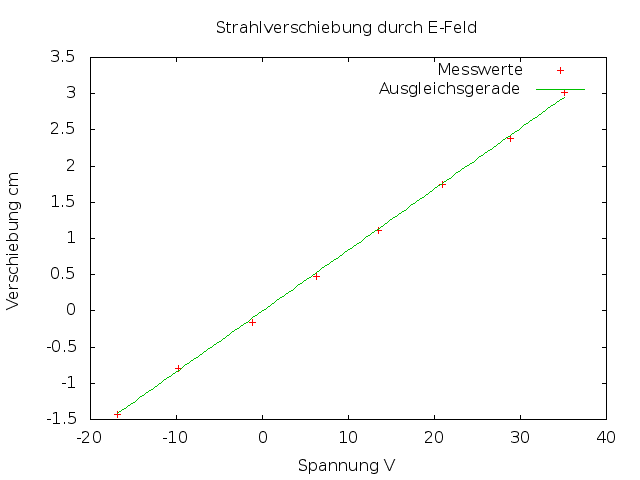
\includegraphics[width=1\textwidth] {pics/400.png}
\centering
\caption{Leuchtfleckverschiebung gegen Ablenkspannung. Hier im Beispiel bei $U_b$ = 400 V}
\end{figure}

\begin{figure}[H]
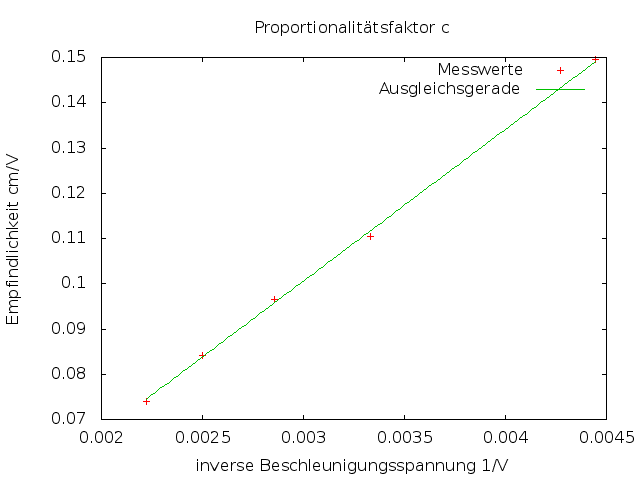
\includegraphics[width=1\textwidth] {pics/proportional.png}
\centering
\caption{Proportionalitätsfaktor c zwischen inverser Beschleunigungsspannung und Empfindlichkeit}
\end{figure}

Der Wert des gewonnenen Faktor $c$ wird nun mit dem aus Gleichung \eqref{} gleichbedeutendem $\frac{pL}{2d}$ verglichen.
Aufgrund des veränderlichen Werts für d wird der Mittelwert der Randwerte für d hergenommen.

\begin{align}
 \left< d \right> = \frac{p_1 \cdot d_1 + (p-p_1) \cdot d_2)}{p} = \frac{1,03\text{cm} \cdot 0,38\text{cm} + 0,87\text{cm} \cdot 0,95\text{cm}}{1,9\text{cm}} = 0,64 \text{cm}
\end{align}

somit ergibt sich

\begin{align}
 \frac{pL}{2d} = \frac{1,9\text{cm} \cdot 14,3\text{cm}}{2 \cdot 0,64\text{cm}} = 42,397 \text{cm}.
\end{align}

Die Abweichung vom ermittelten und erwarteten Wert beträgt $\Delta c = \frac{pL}{2d} - c = 8,855 \text{cm}$ und damit ist
c 26,44 \% größer als der Theoriewert.

\subsection{Frequenz des Sinusgenerators}
Durch Variation der Frequenz der Sägezahnspannung $\nu_{Sae}$, welche an das Plattenpaar für die x-Ablenkung angelegt ist,
werden für rationale Verhältnisse zwischen ihr und der zu untersuchenden Sinusspannung stehende Bilder erzeugt.


\renewcommand{\arraystretch}{1.5}
\begin{table}[h]
 \centering
\begin{tabular}{c|c|c}
n & $\nu_{Sae}$/Hz & $\nu_{Sin}$/Hz\\
\hline
0.5 & 158,921 & 79,461 \\
1 & 79,472 & 79,472 \\
2 & 39,745 & 79,490 \\
3 & 26,500 & 79,500 \\
\hline
$\left< \nu_{Sin} \right>$ &   & 79,481\\
\end{tabular}
 \caption{Frequenz der Sinusspannung aus Frequenz der Sägezahnspannung und Verhältnis n}
\end{table}
\renewcommand{\arraystretch}{1}

Die beste Schätzfunktion für die Standardabweichung ist gegeben durch

\begin{align}
 S = \sqrt{\frac{1}{N(N-1)} \sum_{k=1}^N (\overline{x} - x_k)^2}
\end{align}

und ergibt für die Frequenz der Sinusspannung einen Wert von \newline
$\nu_{Sin} = (79,481 \pm 0,00877) \text{Hz} = 79,481 \cdot (1 \pm 0,00011) \text{Hz}$.

\subsection{Spezifische Ladung des Elektrons}
Im Folgenden soll durch ein transversales Magnetfeld, erzeugt durch ein Helmholtzspulenpaar (Windungszahl N = 20, Radius R = 0,282m), welches in der Flussdichte B 
veränderlich ist, die spezifische Ladung $\frac{C}{kg}$ des Elektrons ermittelt werden. Entsprechend Formel \eqref{} wird
die gemessene Verschiebung in einen linearisierenden Ausdruck $\rho = \frac{D}{L^2 + D^2}$ mit $L=14,3\text{cm}$, sowie die entsprechende
Stromstärke I in die für die Auswertung relevantere Größe B umgeschrieben.

\renewcommand{\arraystretch}{1.2}
\begin{table}[H]
 \begin{tabular}{c|c|c}
  & $U_b$ = 250 V & $U_b$ = 450 V \\
  \hline
  $\rho$[1/cm] & B[mT] & B[mT]\\
  \hline
  0	&0	&0\\
$3.10\cdot10^{-3}$	&0,019	&0,025\\
$6,16\cdot10^{-3}$	&0,038	&0,053\\
$9,15\cdot10^{-3}$	&0,058	&0,076\\
$12,04\cdot10^{-3}$	&0,076	&0,103\\
$14,80\cdot10^{-3}$	&0,097	&0,130\\
$17.40\cdot10^{-3}$	&0,115	&0,156\\
$19,82\cdot10^{-3}$	&0,139	&0,180\\
$22,06\cdot10^{-3}$	&0,156	&0,207\\
 \end{tabular}
 \caption{Verschiebung D durch das von der Stromstärke induzierte Magnetfeld}
\end{table}
\renewcommand{\arraystretch}{1}

\begin{figure}[H]
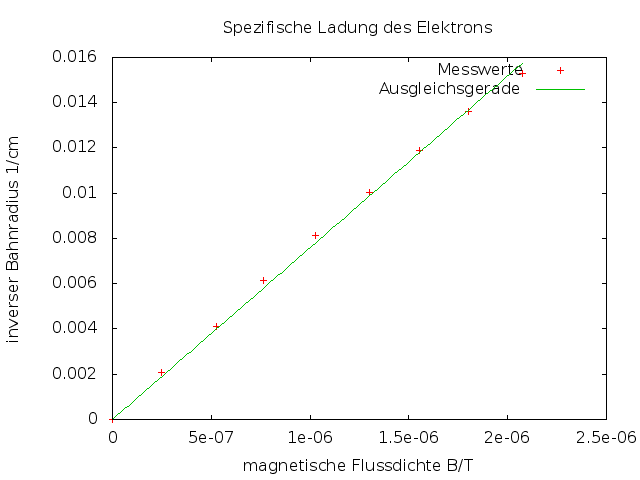
\includegraphics[width=1\textwidth] {pics/spezLadung.png}
\centering
\caption{Proportionalitätsfaktor c zwischen inverser Beschleunigungsspannung und Empfindlichkeit}
\end{figure}

Durch Ausgleichsrechnung durch GNUPLOT ergeben folgende Faktoren:

\begin{align}
& c_{250} = \frac{\rho}{B} = (10061 \pm 109) \text{Tm} = 10061\cdot(1 \pm 0,011) \text{Tm} \\
& c_{450} = \frac{\rho}{B} = (7593,58 \pm 66,56) \text{Tm} = 7593,58\cdot(1 \pm 0,0088) \text{Tm} 
\end{align}

Nun lässt sich endlich die spezifische Ladung des Elektrons über die Beziehung \eqref{} ausdrücken.

\begin{align}
\nonumber
\frac{e_0}{m_0}_{250} &= \left( \frac{D \sqrt{8\cdot U_{250}}}{(L^2+D^2)\cdot B} \right)^2 = (c_{250} \sqrt{8\cdot 250 V})^2 = 2,0245 \cdot 10^{11} \frac{C}{kg} \\
 \nonumber
 \frac{e_0}{m_0}_{450} &= \left( \frac{D \sqrt{8\cdot U_{450}}}{(L^2+D^2)\cdot B} \right)^2 = (c_{450} \sqrt{8\cdot 450 V})^2 = 2,0759 \cdot 10^{11} \frac{C}{kg} \\
 \left< \frac{e_0}{m_0} \right> &= 2,0502 \cdot 10^{11} \frac{C}{kg}
\end{align}

Die Abweichung vom Literaturwert\footnote{Steinhäuser, Niko (2003):Die Spezifische Ladung eines Elektrons} beträgt 
$\Delta \frac{e_0}{m_0} = 2,0502 \cdot 10^{11} \frac{C}{kg} - 1,7588 \cdot 10^{11} \frac{C}{kg} = 0,2914 \cdot 10^{11} \frac{C}{kg}$
und liegt damit 16,67 \% darüber.

\subsection{lokale magnetische Flussdichte des Erdmagnetfelds}
Nach der Drehung des Helmholtzspulenpaars um 90$^\circ$ im Uhrzeigersinn ist der Leuchtfleck durch das Erdmagnetfeld
von der Stelle (0|0) auf (0|-0,635cm) gewandert. Zur Kompensation ist eine Stromstärke von $I_{Komp} = 240$ mA nötig. 
Weiterhin ließ sich der Wert des Inklinationswinkels $\varphi$ = 77$^\circ$ durch einen Kompass ermitteln.\\
Aus Gleichung \eqref{} lässt sich somit das erzeugte Gegenfeld berechnen:

\begin{align}
 \nonumber
 B_{Helmholtz} = B_{hor}= 15,3 \mu\text{T}
 \end{align}
 
Um den Wert des gesamten Magnetfelds an Ort und Zeit des Versuchs zu erhalten, benötigen wir noch die Cosinusbeziehung.

\begin{align}
 B_{hor} = B \cos(\varphi) \Leftrightarrow B = \frac{15,3 \mu\text{T}}{\cos(77^\circ)} = 68,0 \mu\text{T}
\end{align}

\section{Diskussion}
\subsection{Proportionalitätsfaktor c}
Die Abweichung von 26,44\% lässt sich zum Einen sicherlich durch Ungenauigkeit bei der Aufnahme der Messwerte erklären.
So ist die Verschiebung D durch Augenmaß aufgeführt. Zum anderen ist es für den Messprozess erforderlich, dass im 
Kathodenstrahlrohr das Vakuum nicht mehr perfekt ist und es somit zur Abweichung kommt.
\subsection{Spezifische Ladung}
Der Fehler von 16,67\% hat womöglich seine Ursache darin, dass das Magnetfeld des Helmholtzspulenpaars nicht exakt senkrecht
zum Erdmagnetfeld steht. Der zur Verfügung gestellte Kompass zeigt an verschiedenen Stellen im Raum in deutlich verschiedene Richtungen.
Außerdem ist wiedermals zu Berücksichtigen, dass die Verschiebungen durch Augenmaß ermittelt sind. Trotz dessen ist der Wert
durchaus akzeptabel.
\subsection{Erdmagnetfeld}
Der Wert von 68 $\mu$T ist verglichen mit einem Referenzwert von 64 $\mu$T\footnote[2]{Balck, F. (2010), Erdmagnetfeld URL: \href{http://www2.pe.tu-clausthal.de/agbalck/biosensor/erdmagnetfeld.htm}{http://www2.pe.tu-clausthal.de/agbalck/biosensor/erdmagnetfeld.htm}} in Mitteleuropa schon nahezu einstimmig.



% ========================================
%	Literaturverzeichnis
% ========================================

%\bibliographystyle{plainnat}			% Bibliographie-Style auswählen
%\bibliography{BIBDATEI}			% Literaturverzeichnis

% ========================================
%	Das Dokument endent
% ========================================

\end{document}
